\documentclass[11pt, twoside, fleqn]{report}
\usepackage[backend=biber, style=ieee]{biblatex}
\usepackage[parfill, skip=1em]{parskip}
\usepackage[labelfont=bf]{caption}
\usepackage[margin=1in]{geometry}
\usepackage[hidelinks]{hyperref}
\usepackage{amssymb, booktabs, derivative, fancyhdr, float, graphicx, natex, pagecolor, pgfplots, siunitx, tikz}

% background and foreground colors
\definecolor{bgcolor}{HTML}{1e1e2e}
\definecolor{fgcolor}{HTML}{cdd6f4}

% catppuccin palette
\definecolor{p1}{HTML}{cba6f7}
\definecolor{p2}{HTML}{f38ba8}
\definecolor{p3}{HTML}{fab387}
\definecolor{p4}{HTML}{a6e3a1}
\definecolor{p5}{HTML}{89dceb}
\definecolor{p6}{HTML}{89b4fa}

% pagecolor
\pagecolor{bgcolor}
\color{fgcolor}

% biblatex
\addbibresource{references.bib}

% fancyhdr
\renewcommand{\chaptermark}[1]{\markboth{\thechapter\ #1}{}}
\renewcommand{\sectionmark}[1]{\markright{\thesection\ #1}}
\renewcommand{\footrulewidth}{0.4pt}

\fancypagestyle{mystyle}{
    \fancyfoot{}
    \fancyfoot[C]{\thepage}
}

% hyperref
\urlstyle{same}

% pgfplots
\pgfplotsset{compat=newest}

% custom
\newcommand{\dash}{\!-\!}
\newcommand{\state}[2]{\prescript{#1}{}{#2}}

\begin{document}

\pagestyle{empty}

\begin{titlepage}
    \null
    \vspace{\fill}
    \begin{center}
        \let \footnote \thanks
        {\LARGE \textbf{Simulation of Molecular Spectra} \par}
        {\large Theory and Applications}
        \vskip 1.5em
            {\large
                \lineskip .5em
                \begin{tabular}[t]{c}
                    Nathan Phillips
                \end{tabular}\par}
        \vskip 1em
            {\large \today}
        \vskip 2em
    \end{center}
    \vspace{\fill}

    \begin{center}
        {\large{\textbf{Texas A\&M University}} \par}
        {\large{Department of Aerospace Engineering}}
    \end{center}
\end{titlepage}

\tableofcontents
\newpage
\listoffigures
\newpage
\listoftables
\newpage

\pagestyle{mystyle}

\input{chapters/approximations}

\input{chapters/structure}

\input{chapters/intensities}

\input{chapters/numbers}

\input{chapters/hund}

\input{chapters/uncoupling}

\input{chapters/transitions}

\input{chapters/lif}

\input{chapters/lineshapes}

\chapter{Placeholder}

\begin{align*}
    P_{11}(J) & = \nu_0^{(1)} + F_1'(J - 1) - F_1''(J) \\
    Q_{11}(J) & = \nu_0^{(1)} + F_1'(J) - F_1''(J)     \\
    R_{11}(J) & = \nu_0^{(1)} + F_1'(J + 1) - F_1''(J)
\end{align*}

\begin{align*}
    P_{12}(J) & = \nu_0^{(1)} + F_1'(J - 1) - F_2''(J) \\
    Q_{12}(J) & = \nu_0^{(1)} + F_1'(J) - F_2''(J)     \\
    R_{12}(J) & = \nu_0^{(1)} + F_1'(J + 1) - F_2''(J)
\end{align*}

\begin{align*}
    P_{22}(J) & = \nu_0^{(2)} + F_2'(J - 1) - F_2''(J) \\
    Q_{22}(J) & = \nu_0^{(2)} + F_2'(J) - F_2''(J)     \\
    R_{22}(J) & = \nu_0^{(2)} + F_2'(J + 1) - F_2''(J)
\end{align*}

\begin{align*}
    P_{21}(J) & = \nu_0^{(2)} + F_2'(J - 1) - F_1''(J) \\
    Q_{21}(J) & = \nu_0^{(2)} + F_2'(J) - F_1''(J)     \\
    R_{21}(J) & = \nu_0^{(2)} + F_2'(J + 1) - F_1''(J)
\end{align*}

\chapter{Multiplet Term Formulas}

Following info is from \textit{Rotational Structure in the Spectra of Diatomic Molecules} by Kov\'acs.

\section{General Multiplet Term Formulas}

In the following formulae, $B = \bar{B}/hc$, $D = \bar{D}/hc$ (p. 54).

These formulae are valid for any value of $\Lambda$ and $\Sigma$. However, they rarely give values that are compatible with experimental data (p. 57) since they are general in $S$. More useful formulae can be defined that are valid for any $Y$ and $\Lambda$, but fixed in $S$ (meaning different formulae for singlet, doublet, triplet, etc. splittings).

\subsection{Hund's Case (a)}

Equation 2.1.1.9
\begin{align*}
    F_a(\Lambda, S, Y \gg J(J + 1)) & = \nu_0 + A\Lambda\Sigma + B[J(J + 1) - \Omega^2 + S(S + 1) -\Sigma^2] \\
                                    & + H_a^c(\Lambda, S) + H_a^{ss}(\Lambda, S) + H_a^{sr}(\Lambda, S)
\end{align*}

\subsection{Hund's Case (b)}

Equation 2.1.1.10
\begin{align*}
    F_b(\Lambda, S, Y \ll N(N + 1)) & = \nu_0 + B[N(N + 1) - \Lambda^2] + A\Lambda^2\frac{J(J + 1) - N(N + 1) - S(S + 1)}{2N(N + 1)} \\
                                    & + H_b^c(\Lambda) + H_b^{ss}(\Lambda, S) + H_b^{sr}(\Lambda, S)
\end{align*}

\section{Singlet Terms}

For singlet terms, Hund's cases (a) and (b) are the same, and can therefore be obtained from Eq. 2.2.1.9 (by setting $S = \Sigma = 0$, or from 2.1.1.10 (by setting $S = 0$ and $J = N$).

Equation 2.1.2.1
\begin{equation*}
    F(J) = \nu_0 + B[J(J + 1) - \Lambda^2] - D[J(J + 1) - \Lambda^2]^2
\end{equation*}

\section{Triplet Terms}

For $\state{2}{\Sigma}$ terms, $\Lambda = 0$ and $Y = 0$ (p. 63).

Equation 2.1.3.15
\begin{align*}
    F_{J - \tfrac{1}{2}}(N) = F_1(N) & = \nu_0 + B_\Sigma N(N + 1) - D_\Sigma N^2(N + 1)^2 + \tfrac{1}{2}\gamma N      \\
    F_{J + \tfrac{1}{2}}(N) = F_2(N) & = \nu_0 + B_\Sigma N(N + 1) - D_\Sigma N^2(N + 1)^2 - \tfrac{1}{2}\gamma(N + 1)
\end{align*}

\chapter{Intensity Distribution in Rotational Bands}

Following info is from \textit{Rotational Structure in the Spectra of Diatomic Molecules} by Kov\'acs.

\section{Triplet Transitions}

The following equations used in the intensity factors for triplets. For a $\state{3}{\Sigma}\dash\state{3}{\Sigma}$ transition, $\Lambda = 0$. For Hund's case (b), $Y$ can be replaced with $0$ (p. 70).

Equation 2.1.4.9
\begin{align*}
    u_1^\pm(J) & = \sqrt{\Lambda^2Y(Y - 4) + 4J^2} \pm \Lambda(Y - 2)       \\
    u_3^\pm(J) & = \sqrt{\Lambda^2Y(Y - 4) + 4(J + 1)^2} \pm \Lambda(Y - 2)
\end{align*}

Equation 2.1.4.10
\begin{align*}
    C_1(J) & = \Lambda^2Y(Y - 4)(J - \Lambda + 1)(J + \Lambda) + 2(2J + 1)(J - \Lambda)J(J + \Lambda)               \\
    C_2(J) & = \Lambda^2Y(Y - 4) + 4J(J + 1)                                                                        \\
    C_3(J) & = \Lambda^2Y(Y - 4)(J - \Lambda)(J + \Lambda + 1) + 2(2J + 1)(J - \Lambda + 1)(J + 1)(J + \Lambda + 1)
\end{align*}

For a Hund's case (b) $\state{3}{\Sigma}\dash\state{3}{\Sigma}$ transition, these become
\begin{align*}
    u_1^\pm(J) & = 2J       \\
    u_3^\pm(J) & = 2(J + 1)
\end{align*}

And
\begin{align*}
    C_1(J) & = 2J^3(2J + 1)       \\
    C_2(J) & = 4J(J + 1)          \\
    C_3(J) & = 2(J + 1)^3(2J + 1)
\end{align*}

Table 3.8
\begin{table}[H]
    \centering
    \caption{Line strengths of triplet transitions for a Hund's case (b) $\state{3}{\Sigma}\dash\state{3}{\Sigma}$ transition.}
    \begin{tabular}{cc}
        \toprule
        Branches & Line Strength                                                                                                                          \\
        \midrule
        $P_1(J)$ & $\dfrac{J[(J^2 - 1)u'^+_1(J - 1)u''^+_1(J) + (J^2 - 1)u'^-_1(J - 1)u''^-_1(J) + 8J^2(J - 1)^2]^2}{16C'_1(J - 1)C''_1(J)}$              \\
        \addlinespace[0.5em]
        $Q_1(J)$ & $\dfrac{(2J + 1)[-J(J + 1)u'^+_1(J)u''^+_1(J) + J(J + 1)u'^-_1(J)u''^-_1(J)]^2}{16J(J + 1)C'_1(J)C''_1(J)}$                            \\
        \addlinespace[0.5em]
        $R_1(J)$ & $\dfrac{(J + 1)^2[J(J + 2)u'^+_1(J + 1)u''^+_1(J) + J(J + 2)u'^-_1(J + 1)u''^-_1(J) + 8J^2(J + 1)^2]^2}{16(J + 1)C'_1(J + 1)C''_1(J)}$ \\
        \bottomrule
    \end{tabular}
\end{table}

\chapter{Temporary}

\section{Term Values}

Dunham series expansion from Herzberg, p. 108:
\begin{equation*}
    T = \sum_{\ell j}Y_{\ell j}\ab(v + \tfrac{1}{2})^\ell [J(J + 1)]^j
\end{equation*}

Coefficients From Babou, 2009:
\begin{table}[H]
    \centering
    \caption{Dunham Expansion Coefficients}
    \begin{tabular}{c|ccccc}
        \toprule
        $\ell$ & $j = 0$       & $j = 1$         & $j = 2$    & $j = 3$ & $j = 4$ \\
        \midrule
        0      & $Y_{00}$      & $B_e$           & $-D_e$     & $H_e$   & $L_e$   \\
        1      & $-\omega_e$   & $-\alpha_e$     & $-\beta_e$ &         &         \\
        2      & $\omega_ex_e$ & $\gamma_e$      & $-g_e$     &         &         \\
        3      & $\omega_ey_e$ & $\delta_e$      & $-h_e$     &         &         \\
        4      & $\omega_ez_e$ & $\varepsilon_e$ & $-k_e$     &         &         \\
        5      & $\omega_ea_e$ & $\xi_e$         &            &         &         \\
        6      & $\omega_eb_e$ & $\eta_e$        &            &         &         \\
        7      & $\omega_ec_e$ & $\theta_e$      &            &         &         \\
        8      & $\omega_ed_e$ &                 &            &         &         \\
        9      & $\omega_ee_e$ &                 &            &         &         \\
        \bottomrule
    \end{tabular}
\end{table}

Zero-point energy from Herzberg p. 108:
\begin{equation*}
    Y_{00} = \frac{B_e}{4} + \frac{\alpha_e\omega_e}{12B_e} + \frac{\alpha_e^2\omega_e^2}{144B_e^2} - \omega_ex_e
\end{equation*}

From Babou, 2009:
\begin{equation*}
    T = T_e + G + F
\end{equation*}
where
\begin{align*}
    G = \omega_e\ab(v + \tfrac{1}{2}) & - \omega_ex_e\ab(v + \tfrac{1}{2})^2 + \omega_ey_e\ab(v + \tfrac{1}{2})^3 + \omega_ez_e\ab(v + \tfrac{1}{2})^4 + \omega_ea_e\ab(v + \tfrac{1}{2})^5          \\
                                      & + \omega_eb_e\ab(v + \tfrac{1}{2})^6 + \omega_ec_e\ab(v + \tfrac{1}{2})^7 + \omega_ed_e\ab(v + \tfrac{1}{2})^8 + \omega_ee_e\ab(v + \tfrac{1}{2})^9 + \dotsb
\end{align*}
and (generally)
\begin{equation*}
    F = B_vJ(J + 1) + D_v[J(J + 1)]^2 + H_v[J(J + 1)]^3 + \dotsb
\end{equation*}

The rotational constants are
\begin{align*}
    B_v = B_e & - \alpha_e\ab(v + \tfrac{1}{2}) + \gamma_e\ab(v + \tfrac{1}{2})^2 + \delta_e\ab(v + \tfrac{1}{2})^3 + \varepsilon_e\ab(v + \tfrac{1}{2})^4 + \xi_e\ab(v + \tfrac{1}{2})^5 + \eta_e\ab(v + \tfrac{1}{2})^6 \\
              & + \theta_e\ab(v + \tfrac{1}{2})^7 + \dotsb
\end{align*}
and
\begin{equation*}
    D_v = D_e + \beta_e\ab(v + \tfrac{1}{2}) + g_e\ab(v + \tfrac{1}{2})^2 + h_e\ab(v + \tfrac{1}{2})^3 + k_e\ab(v + \tfrac{1}{2})^4 + \dotsb
\end{equation*}
and
\begin{equation*}
    H_v = H_e + \dotsb
\end{equation*}

From \textit{Molecular Spectroscopic Constants of O$_2$ (B$\state{3}{\Sigma}^-_u$): The Upper State of the Schumann--Runge Bands} by Cheung, Eq. (1):
\begin{equation*}
    \sop{H} = B\vb{N}^2 + \tfrac{2}{3}\lambda(3S_z^2 - \vb{S}^2) + \gamma\vb{N}\vdot\vb{S}
\end{equation*}
where
\begin{equation*}
    \vb{N} = \vb{J} - \vb{S}
\end{equation*}

Which can be expressed as (Wilheit, 1969 Eq. 1)
\begin{align*}
    \sop{H} = B\pmx{
    J(J - 1)                           & 0                                        & 0            \\
    (J + 1)(J + 2)                     & 0                                                       \\
    0                                  & 0                                        & J(J + 1)
    }
                                       & + \lambda\pmx{
    \tfrac{-2J}{2J + 1} + \tfrac{2}{3} & \tfrac{2\sqrt{J(J + 1)}}{2J + 1}         & 0            \\
    \tfrac{2\sqrt{J(J + 1)}}{2J + 1}   & \tfrac{-2(J + 1)}{2J + 1} + \tfrac{2}{3} & 0            \\
    0                                  & 0                                        & \tfrac{2}{3}
    }                                                                                            \\
                                       & + \gamma\pmx{
    J - 1                              & 0                                        & 0            \\
    0                                  & -(J + 2)                                 & 0            \\
    0                                  & 0                                        & 1
    }
\end{align*}
where (Krupiene Appendix C)
\begin{align*}
    B       & = B_0 + B_1N(N + 1)             \\
    \lambda & = \lambda_0 + \lambda_1N(N + 1) \\
    \gamma  & = \gamma_0 + \gamma_1N(N + 1)
\end{align*}
Note that $B_1 = -D_0$

Cheung, Table 1:
\begin{equation*}
    x = J(J + 1)
\end{equation*}
and
\begin{equation*}
    F_2 = T + Bx - Dx^2 + \tfrac{2}{3}\lambda - \gamma + \tfrac{2}{3}\lambda_Dx - \gamma_Dx
\end{equation*}
The matrix elements of the Hamiltonian are symmetric
\begin{equation*}
    \bmx{H_{11} & H_{12} \\ H_{21} & H_{22}}
\end{equation*}
where
\begin{align*}
    H_{11} & = T + B(x + 2) - D(x^2 + 8x + 4) - \tfrac{4}{3}\lambda - 2\gamma - \tfrac{4}{3}\lambda_D(x + 2) - 4\gamma_D(x + 1) \\
    H_{12} & = -2\sqrt{x}\ab[B - 2D(x + 1) - \tfrac{\gamma}{2} - \tfrac{2}{3}\lambda_D - \tfrac{1}{2}\gamma_D(x + 4)]           \\
    H_{21} & = H_{12}                                                                                                           \\
    H_{22} & = T + Bx - D(x^2 + 4x) + \tfrac{2}{3}\lambda - \gamma + \tfrac{2}{3}x\lambda_D - 3x\gamma_D
\end{align*}
The eigenvalues are
\begin{align*}
    F_1, F_3 = & -\tfrac{3}{2}\gamma - \tfrac{7}{2}\gamma_D x - 2 \gamma_D - \tfrac{1}{3}\lambda - \tfrac{1}{3}\lambda_D x - \tfrac{4}{3}\lambda_D + B x + B - D x^2 - 6 D x - 2 D + T                     \\
               & \pm \tfrac{1}{6}\bigl(36 \gamma^2 x + 9 \gamma^2 + 72 \gamma \gamma_D x^2 + 306 \gamma \gamma_D x + 72 \gamma \gamma_D + 36 \gamma \lambda + 132 \gamma \lambda_D x + 48 \gamma \lambda_D \\
               & - 144 \gamma B x - 36 \gamma B + 288 \gamma D x^2 + 360 \gamma D x + 72 \gamma D + 36 \gamma_D^2 x^{3} + 297 \gamma_D^2 x^2 + 648 \gamma_D^2 x                                            \\
               & + 144 \gamma_D^2 + 36 \gamma_D \lambda x + 144 \gamma_D \lambda + 132 \gamma_D \lambda_D x^2 + 576 \gamma_D \lambda_D x + 192 \gamma_D \lambda_D - 144 \gamma_D B x^2                     \\
               & - 612 \gamma_D B x - 144 \gamma_D B + 288 \gamma_D D x^{3} + 1512 \gamma_D D x^2 + 1512 \gamma_D D x + 288 \gamma_D D + 36 \lambda^2                                                      \\
               & + 72 \lambda \lambda_D x + 96 \lambda \lambda_D - 72 \lambda B + 144 \lambda D x + 144 \lambda D + 36 \lambda_D^2 x^2 + 160 \lambda_D^2 x + 64 \lambda_D^2                                \\
               & - 264 \lambda_D B x - 96 \lambda_D B + 528 \lambda_D D x^2 + 720 \lambda_D D x + 192 \lambda_D D + 144 B^2 x + 36 B^2                                                                     \\
               & - 576 B D x^2 - 720 B D x - 144 B D + 576 D^2 x^{3} + 1296 D^2 x^2 + 864 D^2 x + 144 D^2\bigr)^{1/2}
\end{align*}

\section{H\"onl--London Factors}

From \textit{H\"onl--London Factors for $\state{3}{\Sigma}^\pm\dash\state{3}{\Sigma}^\pm$ Transitions} by Tatum, Table 1:
\begin{table}[H]
    \centering
    \caption{H\"onl--London Factors for $\state{3}{\Sigma}^\pm\dash\state{3}{\Sigma}^\pm$ Transitions}
    \begin{tabular}{ccc}
        \toprule
        Branch              & Emission                                & Absorption                                 \\
        \midrule
        $P_1$               & $\dfrac{(N' + 1)(2N' + 5)}{2N' + 3}$    & $\dfrac{N''(2N'' + 3)}{2N'' + 1}$          \\
        \addlinespace[0.5em]
        $R_1$               & $\dfrac{N'(2N' + 3)}{2N' + 1}$          & $\dfrac{(N'' + 1)(2N'' + 5)}{2N'' + 3}$    \\
        \addlinespace[0.5em]
        $\state{P}{R}_{13}$ & $\dfrac{1}{(N' + 1)(2N' + 1)(2N' + 3)}$ & $\dfrac{1}{N''(2N'' - 1)(2N'' + 1)}$       \\
        \addlinespace[0.5em]
        $\state{P}{Q}_{12}$ & $\dfrac{1}{N' + 1}$                     & $\dfrac{1}{N''}$                           \\
        \addlinespace[0.5em]
        $P_2$               & $\dfrac{N'(N' + 2)}{N' + 1}$            & $\dfrac{(N'' - 1)(N'' + 1)}{N''}$          \\
        \addlinespace[0.5em]
        $R_2$               & $\dfrac{(N' - 1)(N' + 1)}{N'}$          & $\dfrac{N''(N'' + 2)}{N'' + 1}$            \\
        \addlinespace[0.5em]
        $\state{P}{Q}_{23}$ & $\dfrac{1}{N' + 1}$                     & $\dfrac{1}{N''}$                           \\
        \addlinespace[0.5em]
        $\state{R}{Q}_{21}$ & $\dfrac{1}{N'}$                         & $\dfrac{1}{N'' + 1}$                       \\
        \addlinespace[0.5em]
        $P_3$               & $\dfrac{(N' + 1)(2N' - 1)}{2N' + 1}$    & $\dfrac{N''(2N'' - 3)}{2N'' - 1}$          \\
        \addlinespace[0.5em]
        $R_3$               & $\dfrac{N'(2N' - 3)}{2N' - 1}$          & $\dfrac{(N'' + 1)(2N'' - 1)}{2N'' + 1}$    \\
        \addlinespace[0.5em]
        $\state{R}{Q}_{32}$ & $\dfrac{1}{N'}$                         & $\dfrac{1}{N'' + 1}$                       \\
        \addlinespace[0.5em]
        $\state{R}{P}_{31}$ & $\dfrac{1}{N'(2N' - 1)(2N' + 1)}$       & $\dfrac{1}{(N'' + 1)(2N'' + 1)(2N'' + 3)}$ \\
        \bottomrule
    \end{tabular}
\end{table}

\section{Spectral Lineshapes}

\subsection{Lorentzian Profile}

From \textit{A Student's Guide to Atomic Physics} by Fox, Eq. (3.31) and \textit{Spectroscopy and Optical Diagnostics for Gases} by Hanson, Eq. (8.7):
\begin{equation*}
    \phi_L(\nu) = \frac{1}{2\pi}\frac{\adif{\nu}}{(\nu - \nu_0)^2 + (\adif{\nu}/2)^2}
\end{equation*}

From \textit{A Student's Guide to Atomic Physics} by Fox, Eq. (3.32) and \textit{Spectroscopy and Optical Diagnostics for Gases} by Hanson, Eq. (8.6):
\begin{equation*}
    \adif{\nu} = \frac{1}{2\pi}\ab(\frac{1}{\tau'} + \frac{1}{\tau''})
\end{equation*}

\subsection{Natural Broadening}

From \textit{Spectroscopy and Optical Diagnostics for Gases} by Hanson, Eq. (8.11):
\begin{equation*}
    \adif{\nu}_N = \frac{1}{2\pi}\ab(\sum_k A_{ik} + \sum_k A_{jk})
\end{equation*}

\subsection{Collisional Broadening}

From \textit{A Student's Guide to Atomic Physics} by Fox, Eq. (3.35) and \textit{Spectroscopy and Optical Diagnostics for Gases} by Hanson, Eq. (8.17):
\begin{equation*}
    \adif{\nu}_C = \frac{p\sigma_c}{2\pi}\sqrt{\frac{8}{\pi\mu_{12}k_BT}}
\end{equation*}

From \textit{Spectroscopy and Optical Diagnostics for Gases} by Hanson, Eq. (8.12) and Plasma Physics Slideset 5, page 5:
\begin{equation*}
    \sigma_c = \pi d_{12}^2 = \pi\ab(\frac{d_1 + d_2}{2})^2
\end{equation*}

From \textit{Spectroscopy and Optical Diagnostics for Gases} by Hanson, Eq. (8.15):
\begin{equation*}
    \mu_{12} = \frac{m_1m_2}{m_1 + m_2}
\end{equation*}

\subsection{Gaussian Profile}

From \textit{A Student's Guide to Atomic Physics} by Fox, Eq. (3.42) and \textit{Spectroscopy and Optical Diagnostics for Gases} by Hanson, Eq. (8.22):
\begin{equation*}
    \phi_G(\nu) = \frac{2}{\adif{\nu}}\sqrt{\frac{\ln{2}}{\pi}}\exp\ab[-4\ln{2}\ab(\frac{\nu - \nu_0}{\adif{\nu}})^2]
\end{equation*}

\subsection{Doppler Broadening}

From \textit{A Student's Guide to Atomic Physics} by Fox, Eq. (3.43) and \textit{Spectroscopy and Optical Diagnostics for Gases} by Hanson, Eq. (8.24):
\begin{equation*}
    \adif{\nu}_D = \nu_0\sqrt{\frac{8kT\ln{2}}{mc^2}}
\end{equation*}

\section{Transition Intensities}

\subsection{Inner Product}

From \textit{Introduction to Quantum Mechanics} by Griffiths, Eq. (3.6):
\begin{equation*}
    \ip{f}{g} = \int_a^b \cc{f}g \odif{x}
\end{equation*}

\subsection{Transition Moment}

From Herzberg, Eq. (IV, 67):
\begin{equation*}
    \vb{R} = \int \psi'\vb{M}\psi'' \odif{\tau}
\end{equation*}

From Herzberg, Eq. (VI, 58): (non-degenerate only?)
\begin{equation*}
    \vb{R} = \vb{R}_e^{nm}\vb{R}_v^{v'v''}\vb{R}_r^{J'J''}
\end{equation*}

\section{Partition Functions}

\subsection{General Form}

General form of the Boltzmann population distribution Hanson Eq. (1.11):
\begin{equation*}
    \frac{N_i}{N} = \frac{g_i\exp\ab(-\frac{\varepsilon_i}{kT})}{Q}
\end{equation*}
General form of the partition function Hanson Eq. (1.12):
\begin{equation*}
    Q = \sum_i g_i\exp\ab(-\frac{\varepsilon_i}{kT})
\end{equation*}
The total molecular partition function can be expressed as the product of the individual translational, electronic, vibrational, rotational, and nuclear components for symmetric molecules Hanson Eq. (5.4):
\begin{equation*}
    Q = Q_tQ_eQ_vQ_rQ_n
\end{equation*}

\subsection{Nuclear}

Nuclear partition function for a molecule Hanson Eq. (5.9):
\begin{equation*}
    Q_n = \prod_{i = 1}^L (2I_n + 1)
\end{equation*}

\subsection{Rotational}
Because of the rotational symmetry of certain molecules, a symmetry parameter $\sigma$ must be added to the rotational partition function to account for the multiple molecular orientations that are indistinguishable.
Herzberg Eq. (III, 164):
\begin{equation*}
    Q_r = \frac{1}{\sigma} \sum g_r\exp\ab(-\frac{\varepsilon_r}{kT})
\end{equation*}
The degeneracy of each state is
\begin{equation*}
    g_r = 2J + 1
\end{equation*}
and the rotational energy can be expressed as the term value
\begin{equation*}
    \varepsilon_r = F(J)hc.
\end{equation*}
Therefore, the rotational partition function is
\begin{equation*}
    Q_r = \frac{1}{\sigma} \sum (2J + 1)\exp\ab(-\frac{F(J)hc}{kT}).
\end{equation*}
For sufficiently large $T$ or small $B$,
Rotational partition function for a molecule in the high-temperature limit Hanson Eq. (2.21) and Herzberg Eq. (III, 166):
\begin{equation*}
    Q_r \approx \frac{1}{\sigma} \int_{0}^{\infty} (2J + 1)\exp\ab(-\frac{BJ(J + 1)hc}{kT}) \odif{J} = \frac{1}{\sigma}\frac{kT}{hcB}
\end{equation*}
The Boltzmann fraction is then
\begin{equation*}
    \frac{N_J}{N} = \frac{(2J + 1)\exp\ab(-\frac{F(J)hc}{kT})}{Q_r}
\end{equation*}

\subsection{Effective Rotational}

The effective rotational partition function for symmetric molecules is Hanson Eq. (5.5):
\begin{equation*}
    Q'_r = Q_rQ_n
\end{equation*}
Similarly, the effective rotational degeneracy is Hanson Eq. (5.6):
\begin{equation*}
    g'_r = g_rg_n
\end{equation*}

\subsection{Vibrational}

Herzberg Eq. (III, 159)
\begin{equation*}
    Q_v = \sum g_v\exp\ab(-\frac{\varepsilon_v}{kT})
\end{equation*}
The vibrational degeneracy of each state is
\begin{equation*}
    g_v = 1,
\end{equation*}
and the vibrational energy can be expressed as the term value
\begin{equation*}
    \varepsilon_v = G(v)hc.
\end{equation*}
Therefore, the vibrational partition function is
\begin{equation*}
    Q_v = \sum \exp\ab(-\frac{G(v)hc}{kT}).
\end{equation*}
The Boltzmann fraction is then
\begin{equation*}
    \frac{N_v}{N} = \frac{\exp\ab(-\frac{G(v)hc}{kT})}{Q_v}
\end{equation*}

\subsection{Electronic}

Anderson Eq. (11.56)
\begin{equation*}
    Q_e = \sum g_e\exp\ab(-\frac{\varepsilon}{kT})
\end{equation*}
The electronic degeneracy depends on the individual states. The electronic energy can be expressed as the term value
\begin{equation*}
    \varepsilon_e = T_ehc.
\end{equation*}
Therefore, the electronic partition function is
\begin{equation*}
    Q_e = \sum g_e\exp\ab(-\frac{T_ehc}{kT}).
\end{equation*}

\subsection{Translation}

Anderson Eq. (11.53)
\begin{equation*}
    Q_t = \ab(\frac{2\pi mkT}{h^2})^{3/2}V,
\end{equation*}
where $V$ is the volume of the system.

\section{Rate Equations}

\begin{figure}[H]
    \centering
    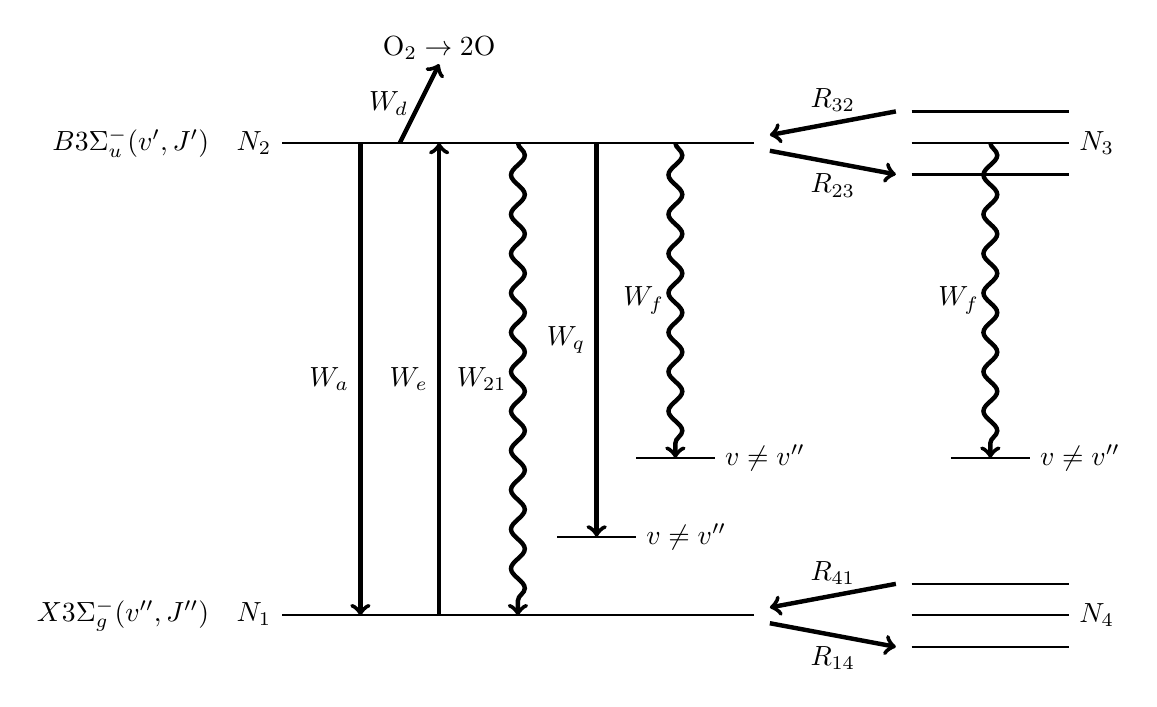
\begin{tikzpicture}
        \draw[thick] (6,0) -- (0,0) node[left] {$X\state{3}{\Sigma}_g^-(v'', J'') \quad N_1$};
        \draw[thick] (6,6) -- (0,6) node[left] {$B\state{3}{\Sigma}_u^-(v', J') \quad N_2$};

        \draw[->,ultra thick] (1,6) -- (1,0) node[midway,left] {$W_a$};
        \draw[->,ultra thick] (1.5,6) -- (2,7) node[midway,left] {$W_d$};
        \node at(2,7.2) {O$_2 \rightarrow 2$O};
        \draw[->,ultra thick] (2,0) -- (2,6) node[midway,left] {$W_e$};
        \draw[->,ultra thick,decorate,decoration={snake,segment length=5mm}] (3,6) -- (3,0) node[midway,left] {$W_{21}$};
        \draw[->,ultra thick] (4,6) -- (4,1) node[midway,left] {$W_q$};
        \draw[thick] (3.5,1) -- (4.5,1) node[right] {$v \neq v''$};
        \draw[->,ultra thick,decorate,decoration={snake, segment length=5mm}] (5,6) -- (5,2) node[midway,left] {$W_f$};
        \draw[thick] (4.5,2) -- (5.5,2) node[right] {$v \neq v''$};

        \draw[<-,ultra thick] (6.2,6.1) -- (7.8,6.4) node[midway,above] {$R_{32}$};
        \draw[thick] (8,6.4) -- (10,6.4);
        \draw[thick] (8,6) -- (10,6) node[right] {$N_3$};
        \draw[thick] (8,5.6) -- (10,5.6);
        \draw[->,ultra thick] (6.2,5.9) -- (7.8,5.6) node[midway,below] {$R_{23}$};

        \draw[->,ultra thick,decorate,decoration={snake,segment length=5mm}] (9,6) -- (9,2) node[midway,left] {$W_f$};
        \draw[thick] (8.5,2) -- (9.5,2) node[right] {$v \neq v''$};

        \draw[<-,ultra thick] (6.2,0.1) -- (7.8,0.4) node[midway,above] {$R_{41}$};
        \draw[thick] (8,0.4) -- (10,0.4);
        \draw[thick] (8,0) -- (10,0) node[right] {$N_4$};
        \draw[thick] (8,-0.4) -- (10,-0.4);
        \draw[->,ultra thick] (6.2,-0.1) -- (7.8,-0.4) node[midway,below] {$R_{14}$};
    \end{tikzpicture}
\end{figure}

\subsection{Four-level LIF}

Gristead thesis, Eq. (2.9)
\begin{align*}
    \odv{N_1}{t} & = -(W_a + R_{14})N_1 + (W_e + W_{21})N_2 + R_{41}N_4                \\
    \odv{N_2}{t} & = W_aN_1 - (W_f + W_d + W_q + W_e + W_{21} + R_{23})N_2 + R_{32}N_3 \\
    \odv{N_3}{t} & = R_{23}N_2 - (W_f + R_{32})N_3                                     \\
    \odv{N_4}{t} & = R_{14}N_1 - R_{41}N_4
\end{align*}
$W_a$ is the laser-stimulated absorption rate, $W_e$ the laser-stimulated emission rate, $W_{21}$ the spontaneous emission rate, $W_d$ the predissociation rate, $W_q$ the collisional quenching rate, $W_f$ the fluorescent radiative decay rate, and $R_{ij}$ the rotational energy transfer rates.

\subsection{Three-level LIF}

Diskin, 1996 Eqs. (1-3)
\begin{align*}
    \odv{N_1}{t} & = -W_aN_1 + (W_e + W_{21})N_2 + W_c\ab(\frac{f_b}{1 - f_b}N_3 - N_1) \\
    \odv{N_2}{t} & = W_aN_1 - (W_e + W_d + W_{21} + W_f + W_q)N_2                       \\
    \odv{N_3}{t} & = -W_c\ab(\frac{f_b}{1 - f_b}N_3 - N_1)
\end{align*}

\appendix
\chapter{Diatomic Constants}
\label{a:diatomic_constants}

\begin{table}[H]
    \centering
    \caption{Diatomic constants for $^{16}\mathrm{O}_2$ \cite{nist:diatomic}.}
    \label{t:diatomic_constants_for_o2}
    \begin{tabular}{cccc}
        \toprule
        Symbol        & \multicolumn{2}{c}{State} & Units                                      \\
        \cmidrule(lr){2-3}
                      & $X~^3\Sigma_g^-$          & $B~^3\Sigma_u^-$        &                  \\
        \midrule
        \multicolumn{4}{c}{\textit{Electronic}}                                                \\
        \cmidrule(lr){1-4}
        $T_e$         & $0$                       & $49793.28$              & $\unit{cm^{-1}}$ \\
        \multicolumn{4}{c}{\textit{Vibrational}}                                               \\
        \cmidrule(lr){1-4}
        $\omega_e$    & $1580.19_3$               & $709.31$                & $\unit{cm^{-1}}$ \\
        $\omega_ex_e$ & $11.98_1$                 & $10.65$                 & $\unit{cm^{-1}}$ \\
        $\omega_ey_e$ & $0.0474_7$                & $-0.139$                & $\unit{cm^{-1}}$ \\
        $\omega_ez_e$ & $-0.00127_3$              & $-$                     & $\unit{cm^{-1}}$ \\
        \multicolumn{4}{c}{\textit{Rotational}}                                                \\
        \cmidrule(lr){1-4}
        $B_e$         & $[1.4376766]$             & $0.8190_2$              & $\unit{cm^{-1}}$ \\
        $\alpha_e$    & $0.0159_3$                & $0.01206$               & $\unit{cm^{-1}}$ \\
        $\gamma_e$    & $-$                       & $-5.5_6\times\num{e-4}$ & $\unit{cm^{-1}}$ \\
        $\delta_e$    & $-$                       & $-$                     & $\unit{cm^{-1}}$ \\
        \multicolumn{4}{c}{\textit{Centrifugal Distortion}}                                    \\
        \cmidrule(lr){1-4}
        $D_e$         &                           &                         & $\unit{cm^{-1}}$ \\
        $\beta_e$     &                           &                         & $\unit{cm^{-1}}$ \\
        \multicolumn{4}{c}{\textit{Spin-Splitting}}                                            \\
        \cmidrule(lr){1-4}
        $\lambda$     &                           &                         & $\unit{cm^{-1}}$ \\
        $\gamma$      &                           &                         & $\unit{cm^{-1}}$ \\
        \multicolumn{4}{c}{\textit{Other}}                                                     \\
        \cmidrule(lr){1-4}
        $H_e$         &                           &                         & $\unit{cm^{-1}}$ \\
        $r_e$         &                           &                         & \AA              \\
        $\nu_{00}$    &                           &                         & $\unit{cm^{-1}}$ \\
        \bottomrule
    \end{tabular}
\end{table}

\chapter{Notation for Diatomic Constants}
\label{a:notation_for_diatomic_constants}

\begin{table}[H]
    \centering
    \caption{Notation for diatomic constants \cite{herzberg:diatomic,nist:sigma1,nist:sigma3}.}
    \label{t:notation}
    \begin{tabular}{clc}
        \toprule
        Symbol        & Definition                                                                  & Units            \\
        \midrule
        \multicolumn{3}{c}{\textit{Electronic}}                                                                        \\
        \cmidrule(lr){1-3}
        $T_e$         & Minimum electronic energy                                                   & $\unit{cm^{-1}}$ \\
        \multicolumn{3}{c}{\textit{Vibrational}}                                                                       \\
        \cmidrule(lr){1-3}
        $G$           & Vibrational energy                                                          & $\unit{cm^{-1}}$ \\
        $\omega_e$    & Vibrational constant - first term                                           & $\unit{cm^{-1}}$ \\
        $\omega_ex_e$ & Vibrational constant - second term                                          & $\unit{cm^{-1}}$ \\
        $\omega_ey_e$ & Vibrational constant - third term                                           & $\unit{cm^{-1}}$ \\
        $\omega_ez_e$ & Vibrational constant - fourth term                                          & $\unit{cm^{-1}}$ \\
        \multicolumn{3}{c}{\textit{Rotational}}                                                                        \\
        \cmidrule(lr){1-3}
        $B_e$         & Rotational constant - equilibrium                                           & $\unit{cm^{-1}}$ \\
        $\alpha_e$    & Rotational constant - first term                                            & $\unit{cm^{-1}}$ \\
        $\gamma_e$    & Rotational constant - second term (rotation-vibration interaction constant) & $\unit{cm^{-1}}$ \\
        $\delta_e$    & Rotational constant - third term                                            & $\unit{cm^{-1}}$ \\
        \multicolumn{3}{c}{\textit{Centrifugal Distortion}}                                                            \\
        \cmidrule(lr){1-3}
        $D_e$         & Centrifugal distortion constant - equilibrium                               & $\unit{cm^{-1}}$ \\
        $\beta_e$     & Centrifugal distortion constant - first term                                & $\unit{cm^{-1}}$ \\
        \multicolumn{3}{c}{\textit{Spin-Splitting}}                                                                    \\
        \cmidrule(lr){1-3}
        $\lambda$     & Spin-spin coupling parameter                                                & $\unit{cm^{-1}}$ \\
        $\gamma$      & Spin-rotation coupling parameter                                            & $\unit{cm^{-1}}$ \\
        \multicolumn{3}{c}{\textit{Other}}                                                                             \\
        \cmidrule(lr){1-3}
        $H_e$         & Sixth-order rotational constant                                             & $\unit{cm^{-1}}$ \\
        $r_e$         & Equilibrium internuclear distance                                           & \AA              \\
        $\nu_{00}$    & Position of $0\dash0$ band                                                  & $\unit{cm^{-1}}$ \\
        \bottomrule
    \end{tabular}
\end{table}

\chapter{Quantum Numbers}
\label{a:quantum_numbers}

\begin{table}[H]
    \centering
    \caption{Various quantum numbers.}
    \label{t:quantum_numbers}
    \begin{tabular}{clc}
        \toprule
        Symbol    & Definition                            & Values                                      \\
        \midrule
        \multicolumn{3}{c}{\textit{Single Electron in Atoms}}                                           \\
        \cmidrule(lr){1-3}
        $n$       & Principal                             & $1, 2, \dotsb$                              \\
        $l$       & Azimuthal                             & $0, 1, \dotsb, (n - 1)$                     \\
        $m_l$     & Magnetic                              & $-l, \dotsb, l$                             \\
        $m_s$     & Spin                                  & $\pm \frac{1}{2}$                           \\
        \multicolumn{3}{c}{\textit{Single Electron in Molecules}}                                       \\
        \cmidrule(lr){1-3}
        $\lambda$ & Orbital Angular Momentum              & $\abs{m_l}$                                 \\
        \multicolumn{3}{c}{\textit{Whole Atoms}}                                                        \\
        \cmidrule(lr){1-3}
        $S$       & Resultant Spin                        & $\sum s_i$                                  \\
        $L$       & Resultant Orbital Angular Momentum    & $\sum l_i$                                  \\
        $J$       & Total Angular Momentum                & $(L + S), (L + S - 1), \dotsb, \abs{L - S}$ \\
        $I$       & Nuclear Spin                          & ?                                           \\
        $F$       & Total Angular Momentum w/ Spin        & $(J + I), (J + I - 1), \dotsb, \abs{J - I}$ \\
        \multicolumn{3}{c}{\textit{Whole Molecules}}                                                    \\
        \cmidrule(lr){1-3}
        $M_L$     & ?                                     & $L, L - 1, \dotsb, -L$                      \\
        $\Lambda$ & Electronic Orbital Angular Momentum   & $0, 1, \dotsb, L$                           \\
        $\Sigma$  & ?                                     & $S, S - 1, \dotsb, -S$                      \\
        $\Omega$  & Resultant Electronic Angular Momentum & $\abs{\Lambda + \Sigma}$                    \\
        $N$       & Total Angular Momentum w/o Spin       & $\Lambda, \Lambda + 1, \dotsb$              \\
        \bottomrule
    \end{tabular}
\end{table}

\chapter{States}
\label{a:states}

\begin{table}[H]
    \centering
    \caption{Various atomic and molecular states.}
    \label{t:states}
    \begin{tabular}{cc}
        \toprule
        Defining Quantum Number & Values                                 \\
        \midrule
        \multicolumn{2}{c}{\textit{Single Electron in Atoms}}            \\
        \cmidrule(lr){1-2}
        $l$                     & s, p, d, f, $\dotsb$                   \\
        \multicolumn{2}{c}{\textit{Single Electron in Molecules}}        \\
        \cmidrule(lr){1-2}
        $\lambda$               & $\sigma, \pi, \delta, \varphi, \dotsb$ \\
        \multicolumn{2}{c}{\textit{Whole Atoms}}                         \\
        \cmidrule(lr){1-2}
        $L$                     & S, P, D, F, $\dotsb$                   \\
        \multicolumn{2}{c}{\textit{Whole Molecules}}                     \\
        \cmidrule(lr){1-2}
        $\Lambda$               & $\Sigma, \Pi, \Delta, \Phi, \dotsb$    \\
        \bottomrule
    \end{tabular}
\end{table}

\printbibliography
\addcontentsline{toc}{chapter}{Bibliography}

\end{document}
